\section{Les cas d'utilisation}
\label{sec:use-cases}

\paragraph{}
Le seul besoin métier est la validation de fichiers Excels contenant des données utiles à l'accomplissement du travail de l'utilisateur. Toutefois, la mise en place d'un site web implique la gestion d'autres aspects comme la sécurité ou l'administration du site web.

\paragraph{}
On distingue trois types d'utilisateurs qui n'ont pas accès aux mêmes fonctionnalités:
\begin{itemize}
    \item Le \textbf{visiteur}: Il n'a accès à rien si ce n'est l'accès à l'authentification afin de gagner les privilèges de l'\textbf{utilisateur}.
    \item L'\textbf{utilisateur}: Il a accès aux fonctionnalités qui font le coeur de l'application. Cette dernière est conçu pour lui.
    \item L'\textbf{administrateur}: Il a tous les droits de l'utilisateur normal avec en plus la possibilité d'accéder aux outils d'administration qui permettent notamment de modifier les paramètres du serveur ainsi que les utilisateurs eux-même.
\end{itemize}

A partir d'ici, je mettrai ces trois termes en gras pour faire explicitement référence aux définitions présentes ci-dessus et afin de les distinguer des termes de la langue française.

\subsection{La liste des cas d'utilisation}
\label{subsec:use-cases-list}

\begin{figure}[ht]
    \centering
    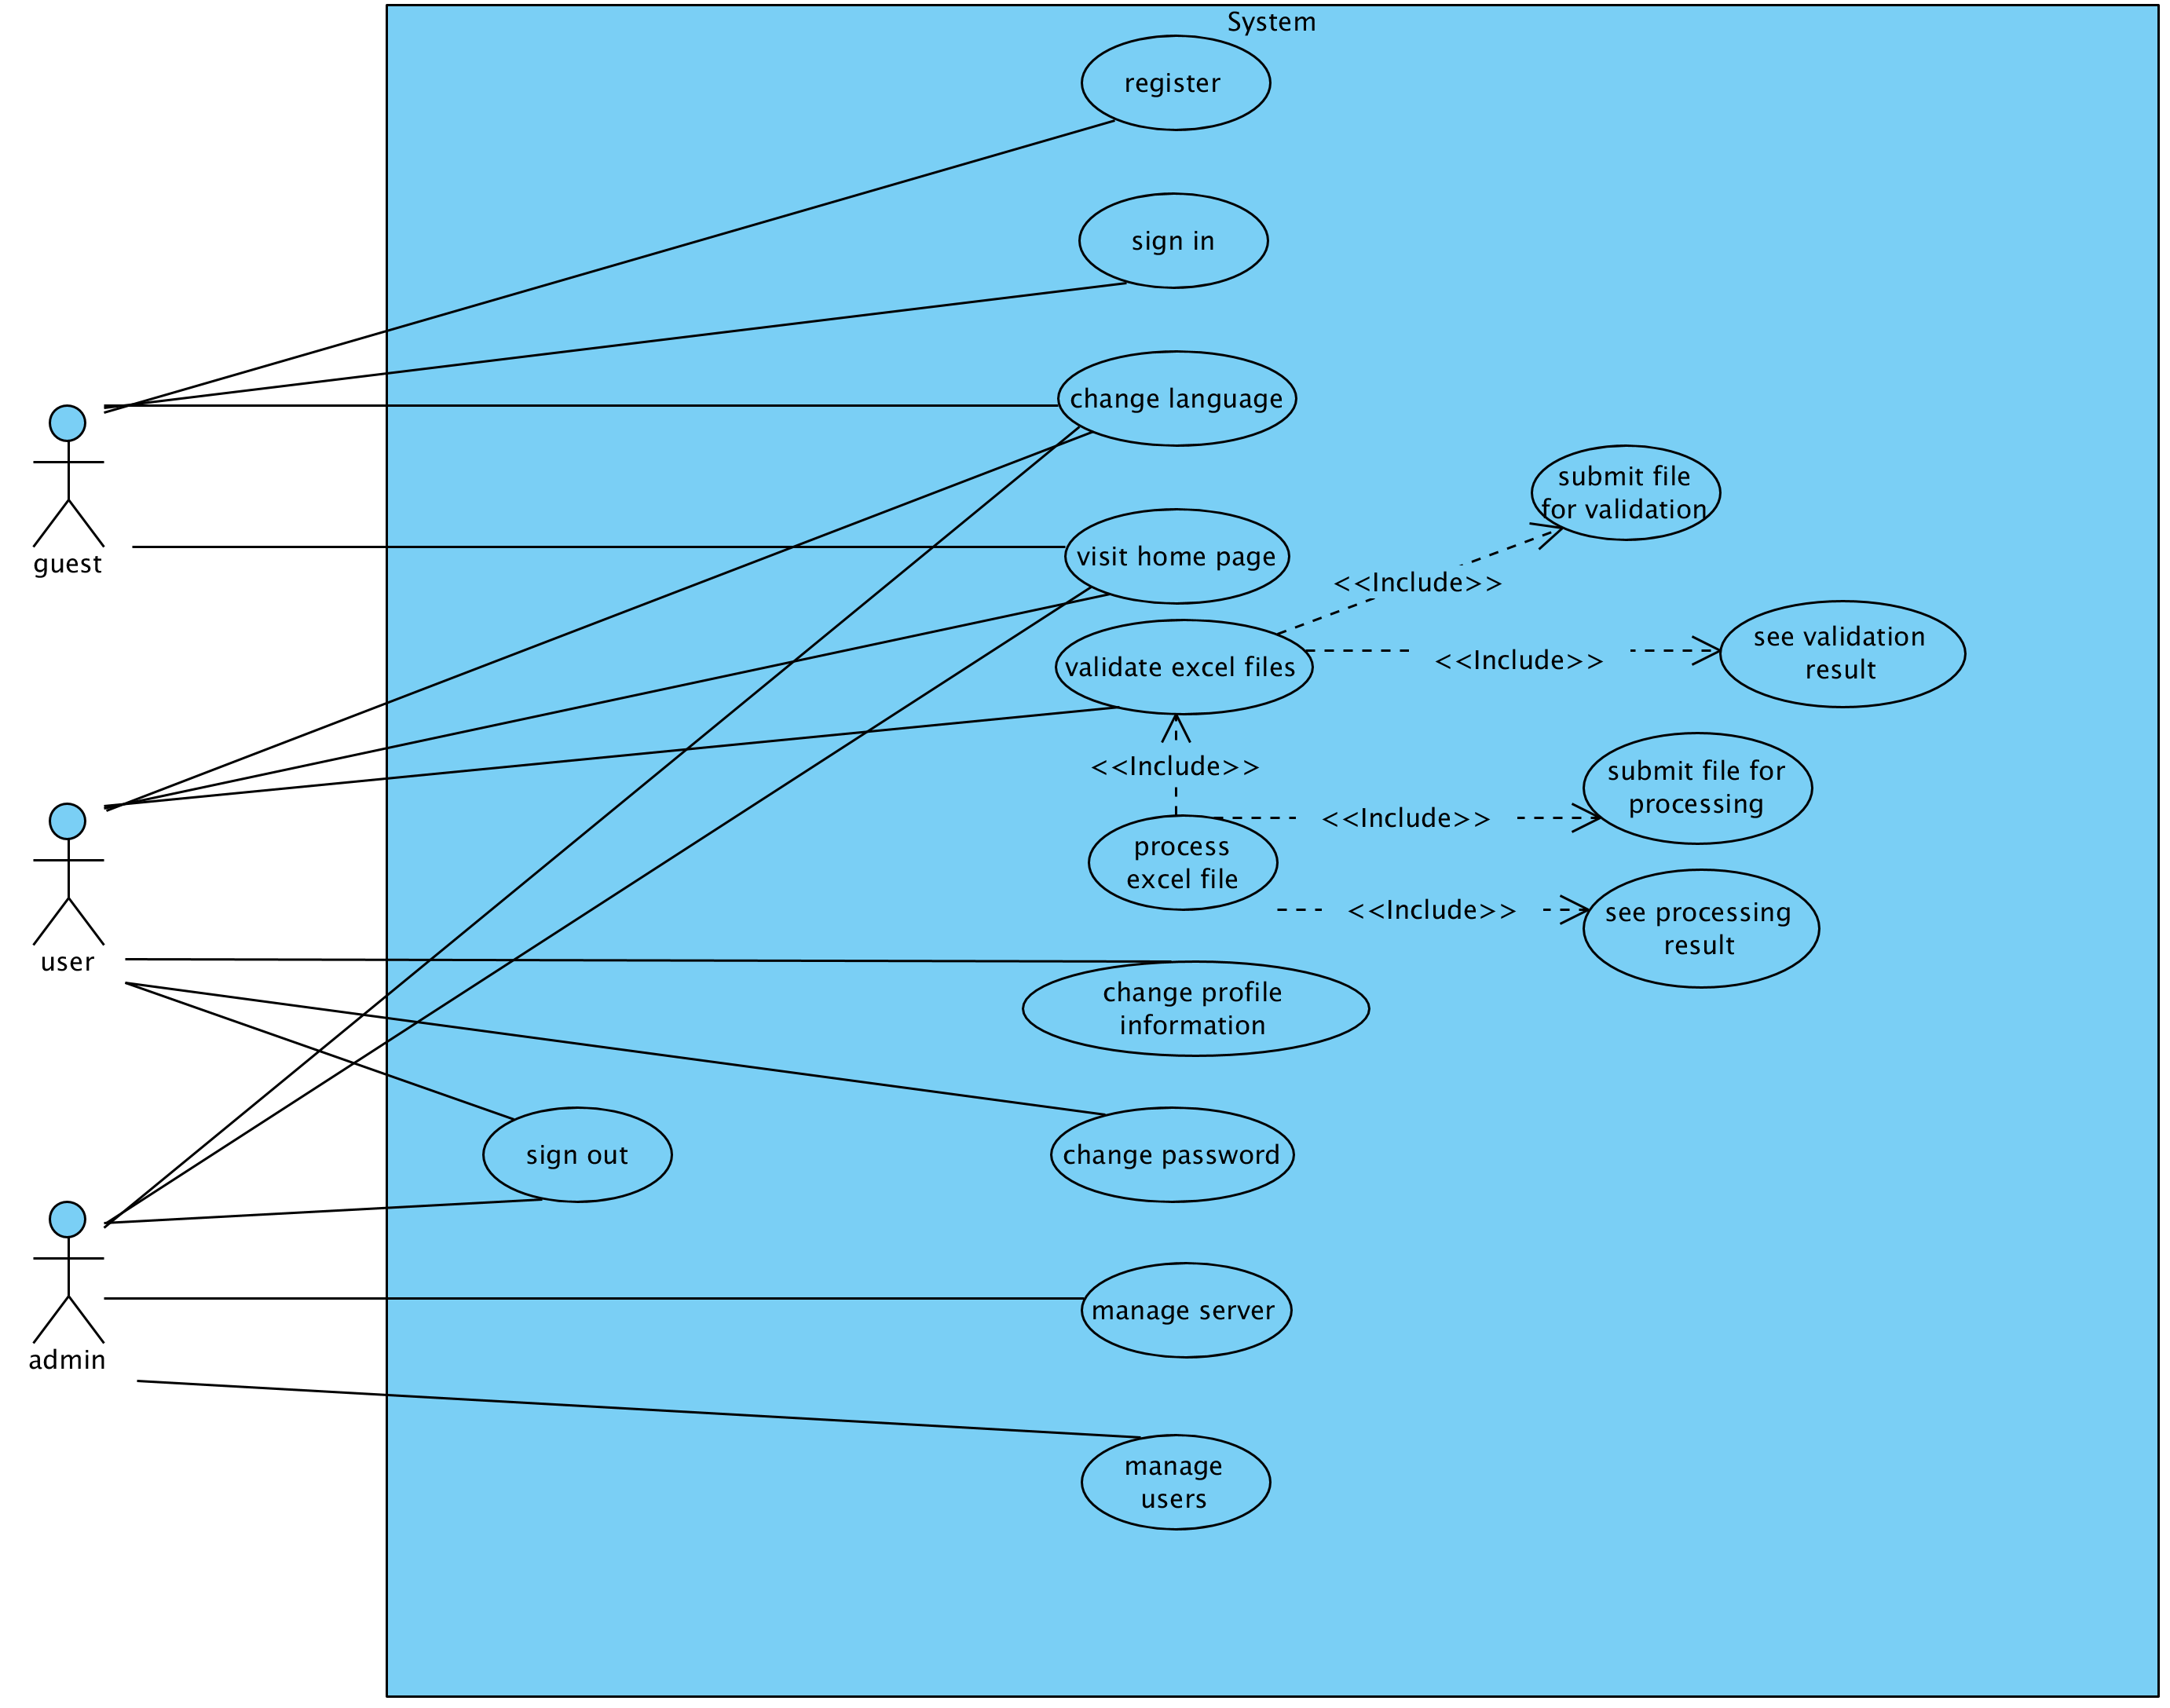
\includegraphics[width=0.8\textwidth]{images/diagrams/use-cases-macro.png}
    \caption{Les cas d'utilisation}
    \label{fig:use-cases-macro}
\end{figure}

\paragraph{}
Le diagramme \ref{fig:use-cases-macro} liste les différents cas d'utilisation et en l'analysant avec attention, on peut observer certains faits qui sont à première vue contre intuitifs.

\paragraph{}
Dans de nombreuses applications, on pourrait considérer une sorte d'héritage entre les différents niveaux de privilèges parmi les utilisateurs. Hors, ce n'est pas le cas ici. En effet, seul le \textbf{visiteur} a accès aux fonctionnalités pour s'enregistrer et se connecter. Plus surprenant, l'\textbf{administrateur} n'a pas accès aux fonctionnalités du coeur de l'application que sont la validation et le traitement des classeurs Excel. Encore plus étonnant, l'administrateur ne peut n'y accéder à son profil, n'y changer son mot de passe.

\begin{figure}[ht]
    \centering
    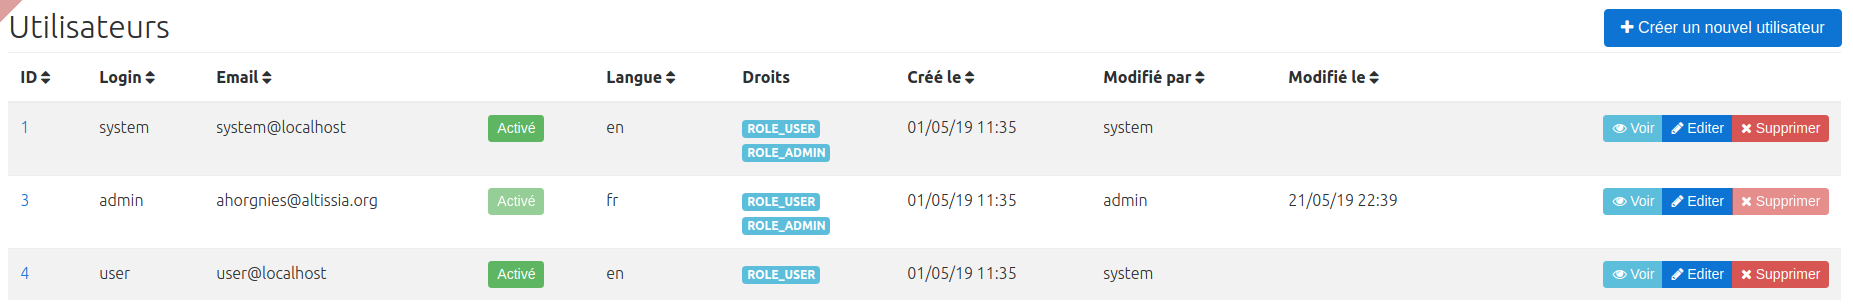
\includegraphics[width=0.8\textwidth]{images/screenshot/screenshot-user-admin-page.png}
    \caption{Une capture d'écran de la page de gestion des utilisateurs}
    \label{fig:user-admin-page}
\end{figure}

\paragraph{}
Cela est du au fait que les permissions sont gérées par un système de licences. Une personne peut cumuler les licences. Ainsi, plutôt que de faire hériter un rôle d'un autre, nous avons choisis de lier les permissions aux licences et de donner autant de licences que nécessaires aux personnes. Cela permet une gestion plus fine des autorisations et aussi plus simple à mettre en place.

Grâce à cela, la nouvelle application peut être déployé avec la base des utilisateurs existante complète sans risquer de compromettre les ressources qu'elle expose. En effet, seuls les personnes qui recevront la licence appropriée auront réellement accès à l'application.

De ce fait, un \textbf{visiteur} n'est pas une personne sans licence mais une personne qui n'a aucune licence adaptée.

Dans les faits, un \textbf{administrateur} aura toujours la licence d'un \textbf{utilisateur}. C'est ce que l'on peut observer sur l'image \ref{fig:user-admin-page}. Il a donc la double casque d'\textbf{administrateur} et d'\textbf{utilisateur}.

\paragraph{}
Le traitement inclue la validation. Bien que ces deux fonctionnalités soient fondamentalement distinctes, nous avons fait le choix d'inclure la validation comme première étape du traitement. Faire ainsi permet d'assurer la validité des données traitées et exclut toute erreur humaine.

\paragraph{}
Une chose qu'il n'est pas possible de voir sur ce diagramme \ref{fig:use-cases-macro} est que la validation et le traitement des classeurs sont des cas d'utilisation abstraits. En effet, il est nécessaire de les spécialiser sans quoi ils ne représentent rien.

Il faut se pencher sur des schémas plus détaillés pour comprendre ce que ces cas d'utilisation couvrent. C'est le sujet de la sous-section \ref{subsec:spreadsheet-use-case}.


\subsection{La validation et le traitement des classeurs Excel}
\label{subsec:spreadsheet-use-case}
